% GNUPLOT: LaTeX picture with Postscript
\begingroup
  \makeatletter
  \providecommand\color[2][]{%
    \GenericError{(gnuplot) \space\space\space\@spaces}{%
      Package color not loaded in conjunction with
      terminal option `colourtext'%
    }{See the gnuplot documentation for explanation.%
    }{Either use 'blacktext' in gnuplot or load the package
      color.sty in LaTeX.}%
    \renewcommand\color[2][]{}%
  }%
  \providecommand\includegraphics[2][]{%
    \GenericError{(gnuplot) \space\space\space\@spaces}{%
      Package graphicx or graphics not loaded%
    }{See the gnuplot documentation for explanation.%
    }{The gnuplot epslatex terminal needs graphicx.sty or graphics.sty.}%
    \renewcommand\includegraphics[2][]{}%
  }%
  \providecommand\rotatebox[2]{#2}%
  \@ifundefined{ifGPcolor}{%
    \newif\ifGPcolor
    \GPcolortrue
  }{}%
  \@ifundefined{ifGPblacktext}{%
    \newif\ifGPblacktext
    \GPblacktextfalse
  }{}%
  % define a \g@addto@macro without @ in the name:
  \let\gplgaddtomacro\g@addto@macro
  % define empty templates for all commands taking text:
  \gdef\gplbacktext{}%
  \gdef\gplfronttext{}%
  \makeatother
  \ifGPblacktext
    % no textcolor at all
    \def\colorrgb#1{}%
    \def\colorgray#1{}%
  \else
    % gray or color?
    \ifGPcolor
      \def\colorrgb#1{\color[rgb]{#1}}%
      \def\colorgray#1{\color[gray]{#1}}%
      \expandafter\def\csname LTw\endcsname{\color{white}}%
      \expandafter\def\csname LTb\endcsname{\color{black}}%
      \expandafter\def\csname LTa\endcsname{\color{black}}%
      \expandafter\def\csname LT0\endcsname{\color[rgb]{1,0,0}}%
      \expandafter\def\csname LT1\endcsname{\color[rgb]{0,1,0}}%
      \expandafter\def\csname LT2\endcsname{\color[rgb]{0,0,1}}%
      \expandafter\def\csname LT3\endcsname{\color[rgb]{1,0,1}}%
      \expandafter\def\csname LT4\endcsname{\color[rgb]{0,1,1}}%
      \expandafter\def\csname LT5\endcsname{\color[rgb]{1,1,0}}%
      \expandafter\def\csname LT6\endcsname{\color[rgb]{0,0,0}}%
      \expandafter\def\csname LT7\endcsname{\color[rgb]{1,0.3,0}}%
      \expandafter\def\csname LT8\endcsname{\color[rgb]{0.5,0.5,0.5}}%
    \else
      % gray
      \def\colorrgb#1{\color{black}}%
      \def\colorgray#1{\color[gray]{#1}}%
      \expandafter\def\csname LTw\endcsname{\color{white}}%
      \expandafter\def\csname LTb\endcsname{\color{black}}%
      \expandafter\def\csname LTa\endcsname{\color{black}}%
      \expandafter\def\csname LT0\endcsname{\color{black}}%
      \expandafter\def\csname LT1\endcsname{\color{black}}%
      \expandafter\def\csname LT2\endcsname{\color{black}}%
      \expandafter\def\csname LT3\endcsname{\color{black}}%
      \expandafter\def\csname LT4\endcsname{\color{black}}%
      \expandafter\def\csname LT5\endcsname{\color{black}}%
      \expandafter\def\csname LT6\endcsname{\color{black}}%
      \expandafter\def\csname LT7\endcsname{\color{black}}%
      \expandafter\def\csname LT8\endcsname{\color{black}}%
    \fi
  \fi
    \setlength{\unitlength}{0.0500bp}%
    \ifx\gptboxheight\undefined%
      \newlength{\gptboxheight}%
      \newlength{\gptboxwidth}%
      \newsavebox{\gptboxtext}%
    \fi%
    \setlength{\fboxrule}{0.5pt}%
    \setlength{\fboxsep}{1pt}%
    \definecolor{tbcol}{rgb}{1,1,1}%
\begin{picture}(7200.00,5040.00)%
    \gplgaddtomacro\gplbacktext{%
      \csname LTb\endcsname%%
      \put(946,1584){\makebox(0,0)[r]{\strut{}$0$}}%
      \csname LTb\endcsname%%
      \put(946,2123){\makebox(0,0)[r]{\strut{}$200$}}%
      \csname LTb\endcsname%%
      \put(946,2662){\makebox(0,0)[r]{\strut{}$400$}}%
      \csname LTb\endcsname%%
      \put(946,3202){\makebox(0,0)[r]{\strut{}$600$}}%
      \csname LTb\endcsname%%
      \put(946,3741){\makebox(0,0)[r]{\strut{}$800$}}%
      \csname LTb\endcsname%%
      \put(946,4280){\makebox(0,0)[r]{\strut{}$1000$}}%
      \csname LTb\endcsname%%
      \put(946,4819){\makebox(0,0)[r]{\strut{}$1200$}}%
      \csname LTb\endcsname%%
      \put(1078,1364){\makebox(0,0){\strut{}$0$}}%
      \csname LTb\endcsname%%
      \put(1700,1364){\makebox(0,0){\strut{}$10$}}%
      \csname LTb\endcsname%%
      \put(2322,1364){\makebox(0,0){\strut{}$20$}}%
      \csname LTb\endcsname%%
      \put(2944,1364){\makebox(0,0){\strut{}$30$}}%
      \csname LTb\endcsname%%
      \put(3567,1364){\makebox(0,0){\strut{}$40$}}%
      \csname LTb\endcsname%%
      \put(4189,1364){\makebox(0,0){\strut{}$50$}}%
      \csname LTb\endcsname%%
      \put(4811,1364){\makebox(0,0){\strut{}$60$}}%
      \csname LTb\endcsname%%
      \put(5433,1364){\makebox(0,0){\strut{}$70$}}%
      \csname LTb\endcsname%%
      \put(6055,1364){\makebox(0,0){\strut{}$80$}}%
      \put(6187,1584){\makebox(0,0)[l]{\strut{}$-2$}}%
      \put(6187,1908){\makebox(0,0)[l]{\strut{}$-1$}}%
      \put(6187,2231){\makebox(0,0)[l]{\strut{}$0$}}%
      \put(6187,2555){\makebox(0,0)[l]{\strut{}$1$}}%
      \put(6187,2878){\makebox(0,0)[l]{\strut{}$2$}}%
      \put(6187,3202){\makebox(0,0)[l]{\strut{}$3$}}%
      \put(6187,3525){\makebox(0,0)[l]{\strut{}$4$}}%
      \put(6187,3849){\makebox(0,0)[l]{\strut{}$5$}}%
      \put(6187,4172){\makebox(0,0)[l]{\strut{}$6$}}%
      \put(6187,4496){\makebox(0,0)[l]{\strut{}$7$}}%
      \put(6187,4819){\makebox(0,0)[l]{\strut{}$8$}}%
    }%
    \gplgaddtomacro\gplfronttext{%
      \csname LTb\endcsname%%
      \put(341,3201){\rotatebox{-270}{\makebox(0,0){\strut{}q (kPa)}}}%
      \put(6693,3201){\rotatebox{-270}{\makebox(0,0){\strut{}$\varepsilon_v$ (\%)}}}%
      \put(3566,1034){\makebox(0,0){\strut{}$\varepsilon_{yy}$ (\%)}}%
      \csname LTb\endcsname%%
      \put(2711,833){\makebox(0,0)[r]{\strut{}$I = 1 \times 10^{-4}$}}%
      \csname LTb\endcsname%%
      \put(2711,613){\makebox(0,0)[r]{\strut{}$I = 1 \times 10^{-3}$}}%
      \csname LTb\endcsname%%
      \put(2711,393){\makebox(0,0)[r]{\strut{}$I = 2 \times 10^{-3}$}}%
      \csname LTb\endcsname%%
      \put(2711,173){\makebox(0,0)[r]{\strut{}$I = 4 \times 10^{-3}$}}%
      \csname LTb\endcsname%%
      \put(5150,833){\makebox(0,0)[r]{\strut{}$I = 6 \times 10^{-3}$}}%
      \csname LTb\endcsname%%
      \put(5150,613){\makebox(0,0)[r]{\strut{}$I = 8 \times 10^{-3}$}}%
      \csname LTb\endcsname%%
      \put(5150,393){\makebox(0,0)[r]{\strut{}$I = 1 \times 10^{-2}$}}%
    }%
    \gplbacktext
    \put(0,0){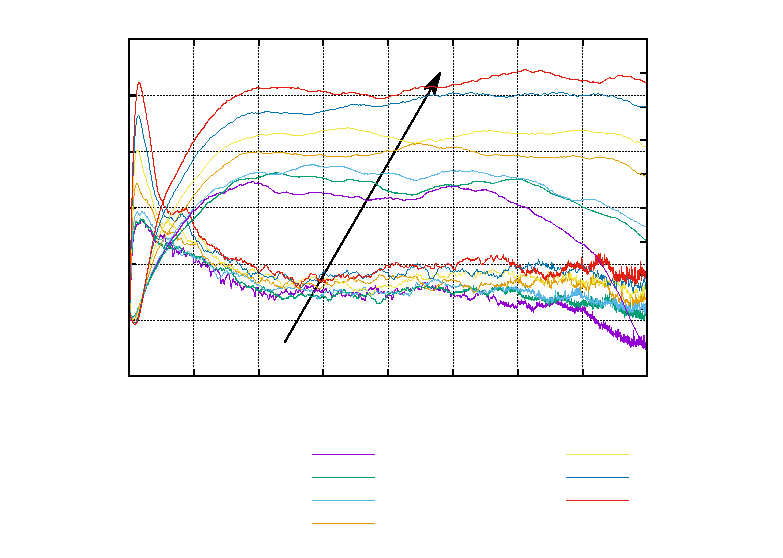
\includegraphics[width={360.00bp},height={252.00bp}]{./Test}}%
    \gplfronttext
  \end{picture}%
\endgroup
